\subsection{Application} \label{sec:application}
We demonstrate POOL by using it to find short peptides that are \enquote{Sfp-specific hits} and \enquote{AcpS-specific hits}. 
We show this application is an instance of the more general problem discussed above. First we look at \enquote{Sfp-specific hit}, for a peptide $e$, let $y(e) = 1$ if it is \enquote{Sfp-specific hit}, since we are looking for short peptides, let the utility function $f(e)$ be negative the length of $e$, and now the problem is the same as \eqref{eq:general problem}. For \enquote{AcpS-specific hits}, we simply modify the definition of $y(e)=1$.

\subsubsection{Performance of Machine Learning Model} \label{sec:application_roc}
We use the machine learning model described in \ref{sec:stat model} to predict $y(e)$. 
As described above, this model represents peptides through \enquote{features}, which summarize properties of interest of a peptide. The feature in our application is designed as follows: since the chemoenzymatic reaction only happens at position containing Serine within the peptide, we are looking for the peptides containing exactly one Serine in the sequence. We use Serine as the origin, and label positions of other amino acids in the sequence by counting how far away it is from the origin and whether it is on the side of C-terminus or N-terminus. Each position encodes one feature, which is determined by the type of amino acid residing in this position. In this application, to reduce dimensionality of the feature space, we group the 20 standard amino acids into 8 classes according to their similarity, and the feature values for the amino acids belonging to the same class are the same. The grouping detail is shown in Table \ref{table:reduced aa}. For example, a sequence X-X-X-S-X-X, where S represents Serine and X represents amino acid alphabet, in feature representation can be written as N3-N2-N1-S-C1-C2, where N\# and C\# are grouping class values for amino acids in the corresponding positions.

We use the constructed features to train the model described in \ref{sec:stat model}. Our dataset 


Over the past two years, we performed 5 rounds of experiments, in which four experiments tested 2022 peptides for Sfp labeling / ACPH unlabeling activity and AcpS labeling / ACPH unlabeling activity, while one experiment in the early stage of the project tested 580 peptides only for Sfp labeling / ACPH unlabeling activity. For the 580 peptides that were only tested Sfp labeling / ACPH unlabeling activity, we do not have information on their specific labeling activity, 


Since we are looking at the peptide activity for three enzymes: Sfp, AcpS and ACPH, and we assume their labeling / unlabeling activity is independent, we train three separate prediction models, and use the method in \ref{sec:extension} to combine the models and predict whether a peptide is \enquote{Sfp-specific hit} or \enquote{AcpS-specific hit}. To validate our model, we performed cross validation and plot receiver operating characteristic (ROC) curve, as shown in Figure~\ref{fig:ROC}, which is typically used to benchmark performance of binary classifiers. 

\begin{figure}[hpt] 
\center
\begin{subfigure}[b]{0.3\linewidth}
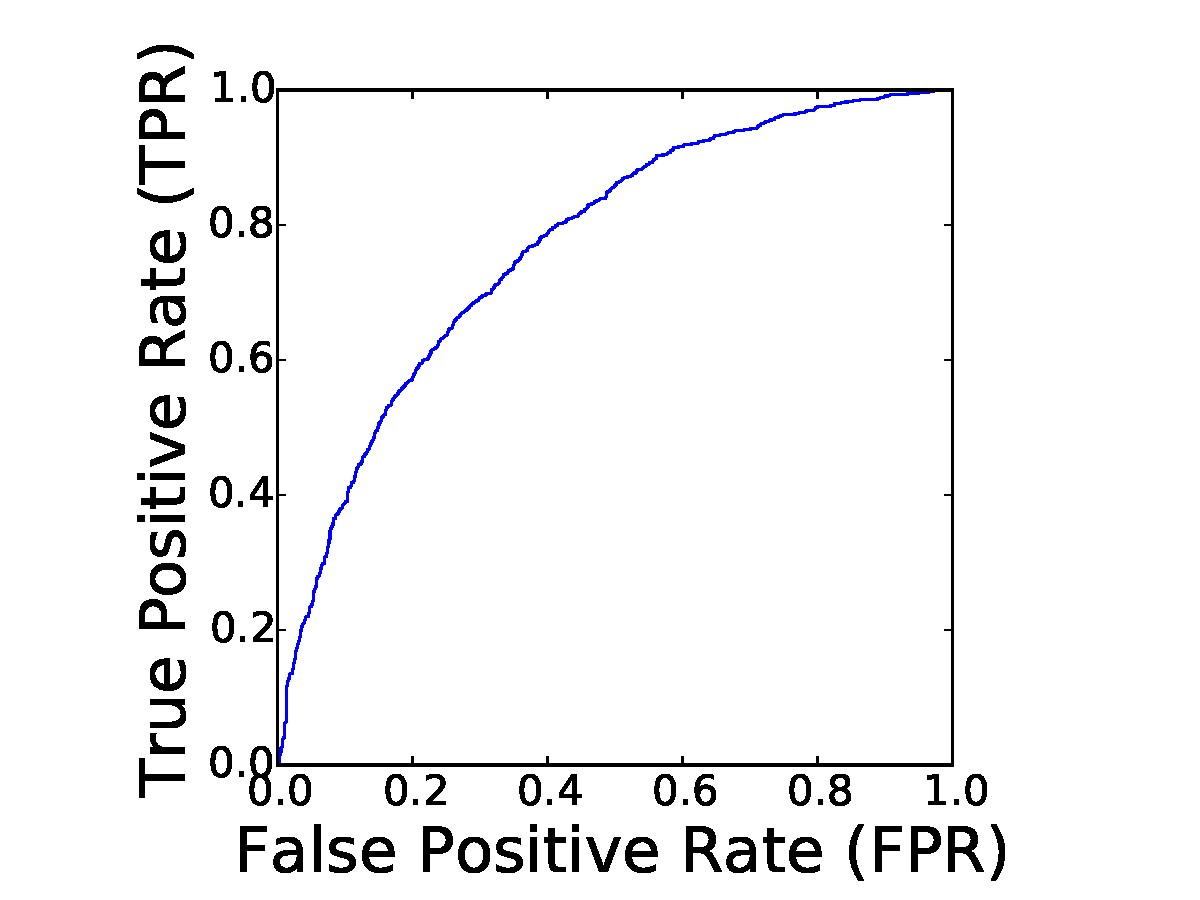
\includegraphics[width=\textwidth]{pic/ROC_sfp.pdf}
\caption{prediction of Sfp labeling activity}
\end{subfigure}
\begin{subfigure}[b]{0.3\linewidth}
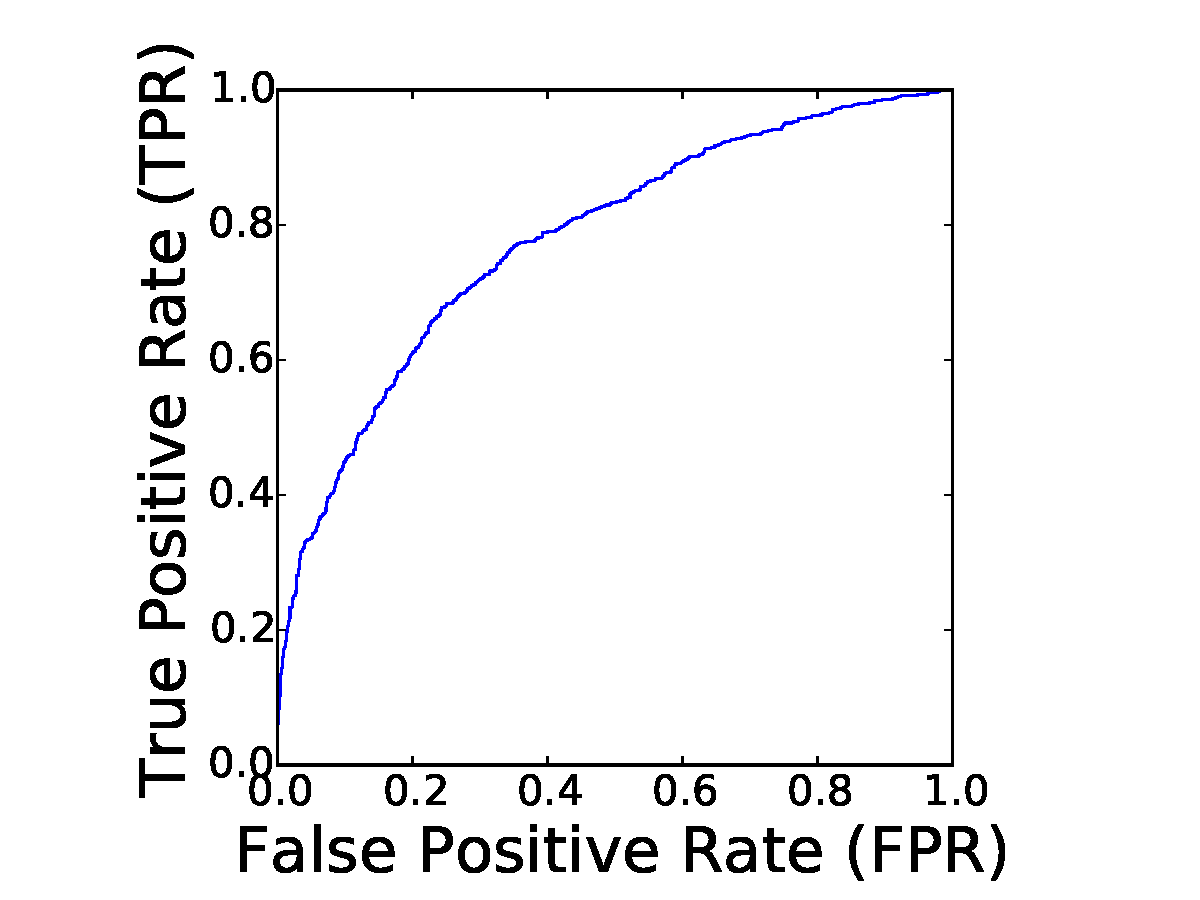
\includegraphics[width=\textwidth]{pic/ROC_AcpS.pdf}
\caption{prediction of AcpS labeling activity}
\end{subfigure}
\begin{subfigure}[b]{0.3\linewidth}
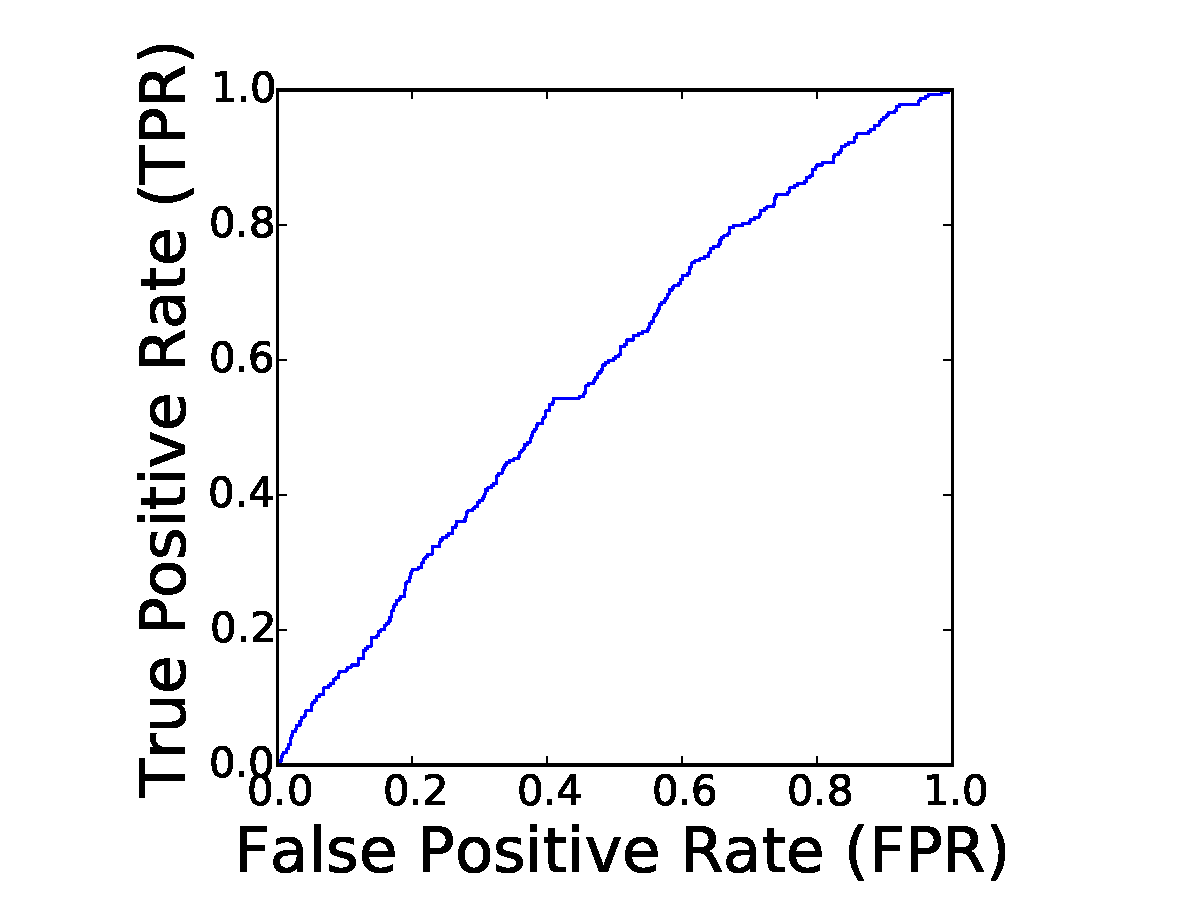
\includegraphics[width=\textwidth]{pic/ROC_PfAcpH.pdf}
\caption{prediction of ACPH unlabeling activity}
\end{subfigure}
\caption{ ROC curve generated by cross validation on all peptides tested so far, which contains Sfp activity for 2602 peptides, AcpS activity for 2022 peptides and ACPH activity for 1380 peptides.}
\label{fig:ROC}
\end{figure}

The classifier performs well if the ROC curve points toward upper left corner, and has no prediction power if the curve is a straight line between $(0,0)$ and $(1,1)$. From the plots we can see the models predicting Sfp and AcpS activity perform very well, but the model predicting ACPH activity has less indicating power.


\subsubsection{Comparison of POOL vs. existing methods}
To illustrate performance of our approach versus existing methods, we simulate a scenario which is very close to our real application, and compare the quality of recommended peptides generated by each method. To simulate a scenario, we used result of all tested peptides to train the model, like we did in \ref{sec:application_roc}, and treat it as \enquote{oracle}, i.e., whether a peptide is a hit or not is completely determined by this trained model. Then we only reveal part of the data to the competing methods, let them generate recommended peptides, and use \enquote{oracle} to evaluate quality of the recommendations produced by the methods. In this experiment, we revealed test result from the first two rounds of experiments, which contain Sfp activity for 847 peptides, AcpS activity for 267 peptides and ACPH activity for 452 peptides. There are only four \enquote{Sfp-specific hits} and one \enquote{AcpS-specific hit} in this revealed dataset. We compare the performance of three methods: they are POOL, which is our proposed approach; predict-then-optimize, discussed in \ref{sec:existing approaches}; mutation method, which is to generate new peptides by mutating existing hits. Each method generates 100 peptides, and we evaluate the quality by calculating the probability of at least one of the recommended peptides is a hit according to \enquote{oracle}. The benchmark plot is shown in Figure~\ref{fig:benchmark}.
\begin{figure}[hpt] 
\center
\begin{subfigure}[b]{0.46\linewidth}
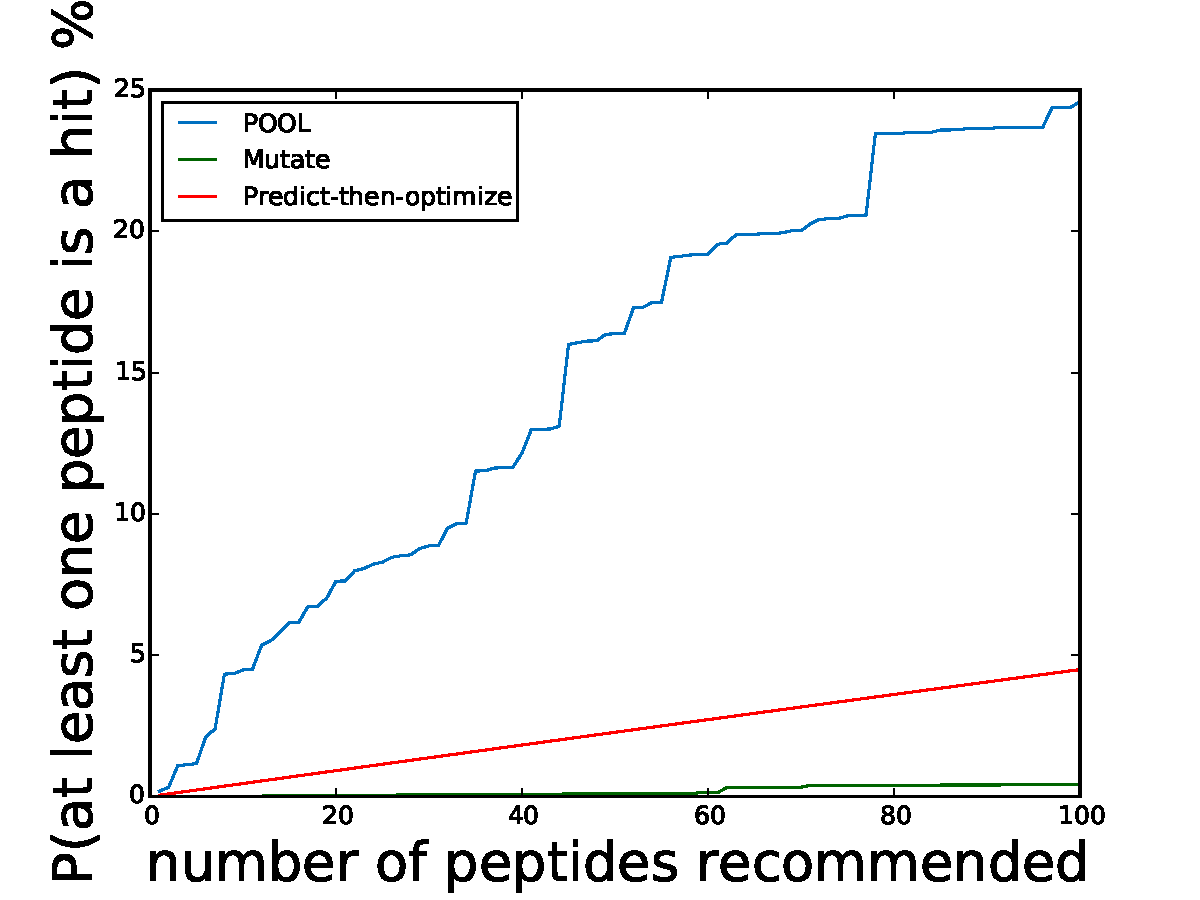
\includegraphics[width=\textwidth]{pic/benchmark_type1.pdf}
\caption{\enquote{Sfp-specific hit}}
\end{subfigure}
\begin{subfigure}[b]{0.46\linewidth}
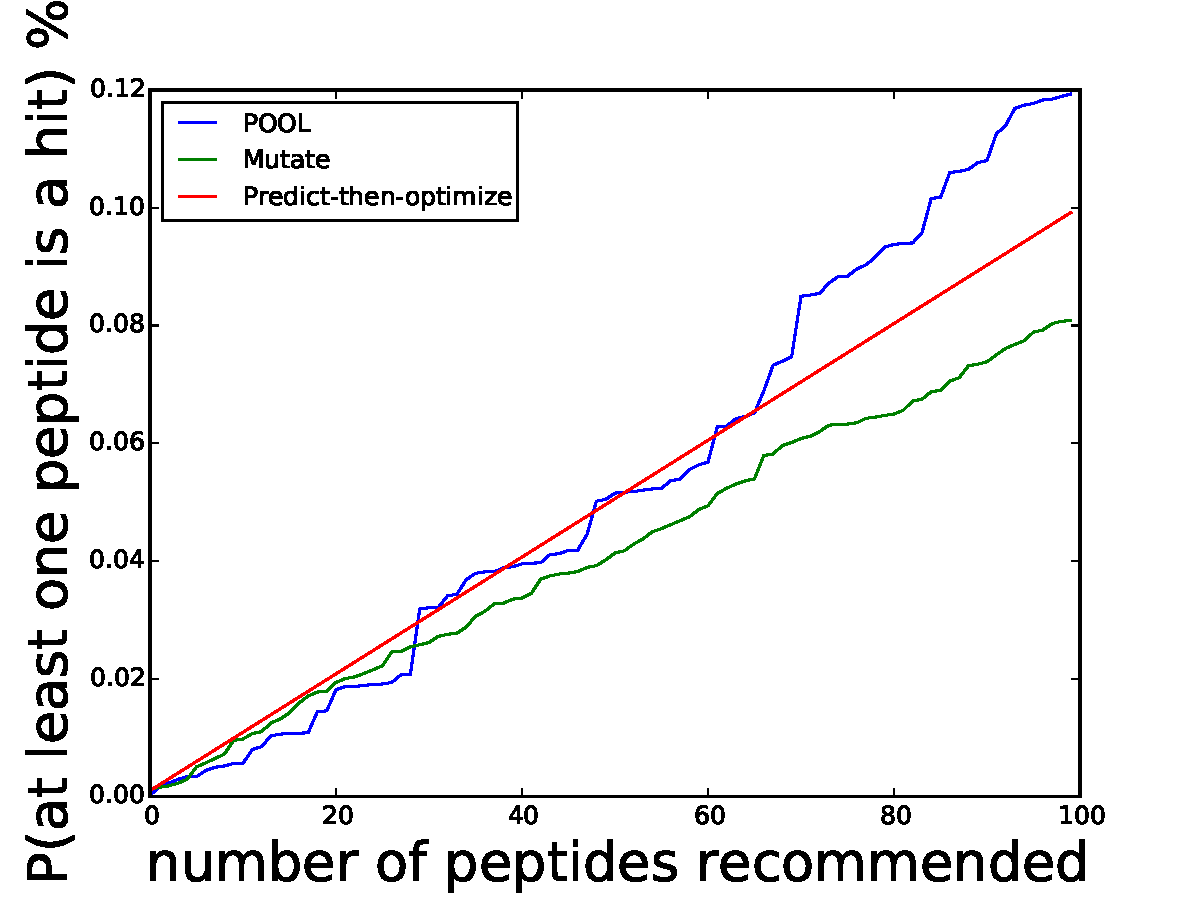
\includegraphics[width=\textwidth]{pic/benchmark_type2.pdf}
\caption{\enquote{AcpS-specific hit}}
\end{subfigure}
\caption{Comparison of quality of recommended peptides by POOL, mutation method and predict-then-optimize approach.}
\label{fig:benchmark}
\end{figure}

From the benchmark we can see POOL beats the other two methods by a significant margin in searching \enquote{Sfp-specific hits}. In the search of \enquote{AcpS-specific hits}, all three methods have similar performance, with POOL achieving a little better, but the recommended peptides have a very low probability that at least one of them is actually a hit according to \enquote{oracle}. This is because the methods only observed one \enquote{AcpS-specific hit}, and it is too hard for the methods to provide high quality peptides given this little information. 